

\documentclass[10pt,journal,compsoc]{IEEEtran}

\usepackage[pdftex]{graphicx}    
\usepackage{cite}
\hyphenation{op-tical net-works semi-conduc-tor}


\begin{document}

\title{Where-Am-I}

\author{Abanob Effat}

\markboth{Localization project, Robotics Nanodegree Program, Udacity}%
{}
\IEEEtitleabstractindextext{%

\begin{abstract}
This project Solves one of the major problems in autonomous robots which is it's location, this project uses two robots to solve the localization problem in known environment using Gazebo and Rviz to simulate the process
\end{abstract}

% Note that keywords are not normally used for peerreview papers.
\begin{IEEEkeywords}
Robot, IEEEtran, Udacity, \LaTeX, Localization.
\end{IEEEkeywords}}


\maketitle
\IEEEdisplaynontitleabstractindextext
\IEEEpeerreviewmaketitle
\section{Introduction}
\label{sec:introduction}

\IEEEPARstart{T}{he} localization problem is one of the major problems that robots must solve dependently as the robot must know it's location because some tasks may be very hard if the robot didn't learn how to tell it's location, Here i am solving the localization problem of a know environment using advanced monte carlo localization.





\section{Background}
As from the above i am solving the localization problem in a know environment but the sensors contain some noise so i am using some techniques to solve this issue.

\subsection{Kalman Filters}
Kalman Filters is used to come over noisy measurements and to estimate the location of the robot. There are two steps in Kalman Filters. They are predict and update. Predict step calculate the position after movement is done and the update step uses the measurements to update the location.
Kalman filters is constrained to Gaussian distributions to work. Therefore only linear operations are allowed. \\
Since the robot model is not linear, there is a need for converting from nonlinear equations to linear equations. Taylor Series is the method for linear approximation. By applying linearity, the Kalman Filter become Extended Kalman Filter. 


\subsection{Particle Filters}
Monte Carlo Localization,First it defines particles that predict the robot position then After motion and position of each particle updates, the uncertainty increases but after the measurements from the sensors, And finally another update is done to decrease the uncertainty.


\subsection{Comparison / Contrast}
Particle Filter can work with any distribution while Kalman Filter only works with a Gaussian distribution. Particle Filter takes raw measurements; however, Kalman Filter requires known places. The posterior is particles for Particle Filter and Gaussian for Kalman Filter. Kalman Filter is more efficient and provides more resolution; on the other hand Particle Filter is easier to implement and more robust. Only Particle Filter has Memory and Resolution control and can provide a solution for Glocal Localization.

\section{Simulations}
The simulations are Gazebo that provide the environment to simulate the two robots rviz to control over each robot and get visual all the data and both these simulations run on ROS framework, The ROS packages are AMCL, move base, map server, and navigation.

\subsection{Achievements}
Both robots could reach the goal but udacity robot went at first to wrong path but my robot didn't and reached the goal position faster.

% Robot Models
\subsection{Benchmark Model}
\subsubsection{Model design}
The main parts of the robot provided by udacity is the chassis. It has rectangular box with dimensions 0.4 x 0.2 x 0.1. It has two casters to overcome the balancing problem, one at -0.15 0 -0.05 and the other at 0.15 0 -0.05. There are two wheels connected to the chassis at 0 -0.15 0 and 0 +0.15 0. 
The laser sensor located at position relative to the chassis 0.15 0 0.085. It has a cubic shape with length 0.1. The camera sensor is connected to the chassis at 0.2 0 0, and it has a cubic shape with lenght 0.05.
The difference between the my robot and the Udacity robot is the a link. The camera and the laser sensors are connected to this link. The link has the dimensions of 0.5 0.01 0.02. It is connected to the chassis at location 0 0 0.075. The camera is connected to sensor\textunderscore link at 0.175 0 0 and the laser sensor connected to the at 0 0 0.05.
\begin{figure}[thpb]
      \centering
      \includegraphics[width=\linewidth]{fig/fin_bot.jpg}
      \caption{bot design}
\end{figure}

\subsubsection{Packages Used}
Packages used for ROS kinetic aree:
\begin{itemize}
\item ros-kinetic-navigation
\item ros-kinetic-map-server
\item ros-kinetic-move-base
\item ros-kinetic-amcl
\end{itemize}

\begin{table}[h]
\caption{Parameter Differences Between Udacity Bot and bot}
\label{table:params_ubot_xbot}
\begin{center}
\begin{tabular}{|c||c||c||c|}
\hline
File or Pkg & Parameter & Udacity Bot & bot\\
\hline
AMCL & min\textunderscore particles & 15 & 100 \\
\hline
AMCL & max\textunderscore particles & 250 & 1000 \\
\hline
Common & obstacle\textunderscore range & 5.0 & 6.0 \\
\hline
Common & raytrace\textunderscore range & 6.0 & 9.0 \\
\hline
Common & inflation\textunderscore radius & 0.5 & 1.0 \\
\hline
Common & robot\textunderscore radius & N/A & 0.5 \\
\hline
Global & update\textunderscore frequency & 5.0 & 3.0 \\
\hline
Global & publish\textunderscore frequency & 5.0 & 3.0 \\
\hline
Local & update\textunderscore frequency & 5.0 & 1.0 \\
\hline
Local & publish\textunderscore frequency & 5.0 & 1.0 \\
\hline
Local & width & 40.0 & 3.0 \\
\hline
Local & height & 40.0 & 3.0 \\
\hline
Local & resolution & 0.05 & 0.01 \\
\hline
\end{tabular}
\end{center}
\end{table}
\begin{figure}[thpb]
      \centering
      \includegraphics[width=\linewidth]{fig/node1.jpg}
      \caption{bot Graph}
\end{figure}
\begin{figure}[thpb]
      \centering
      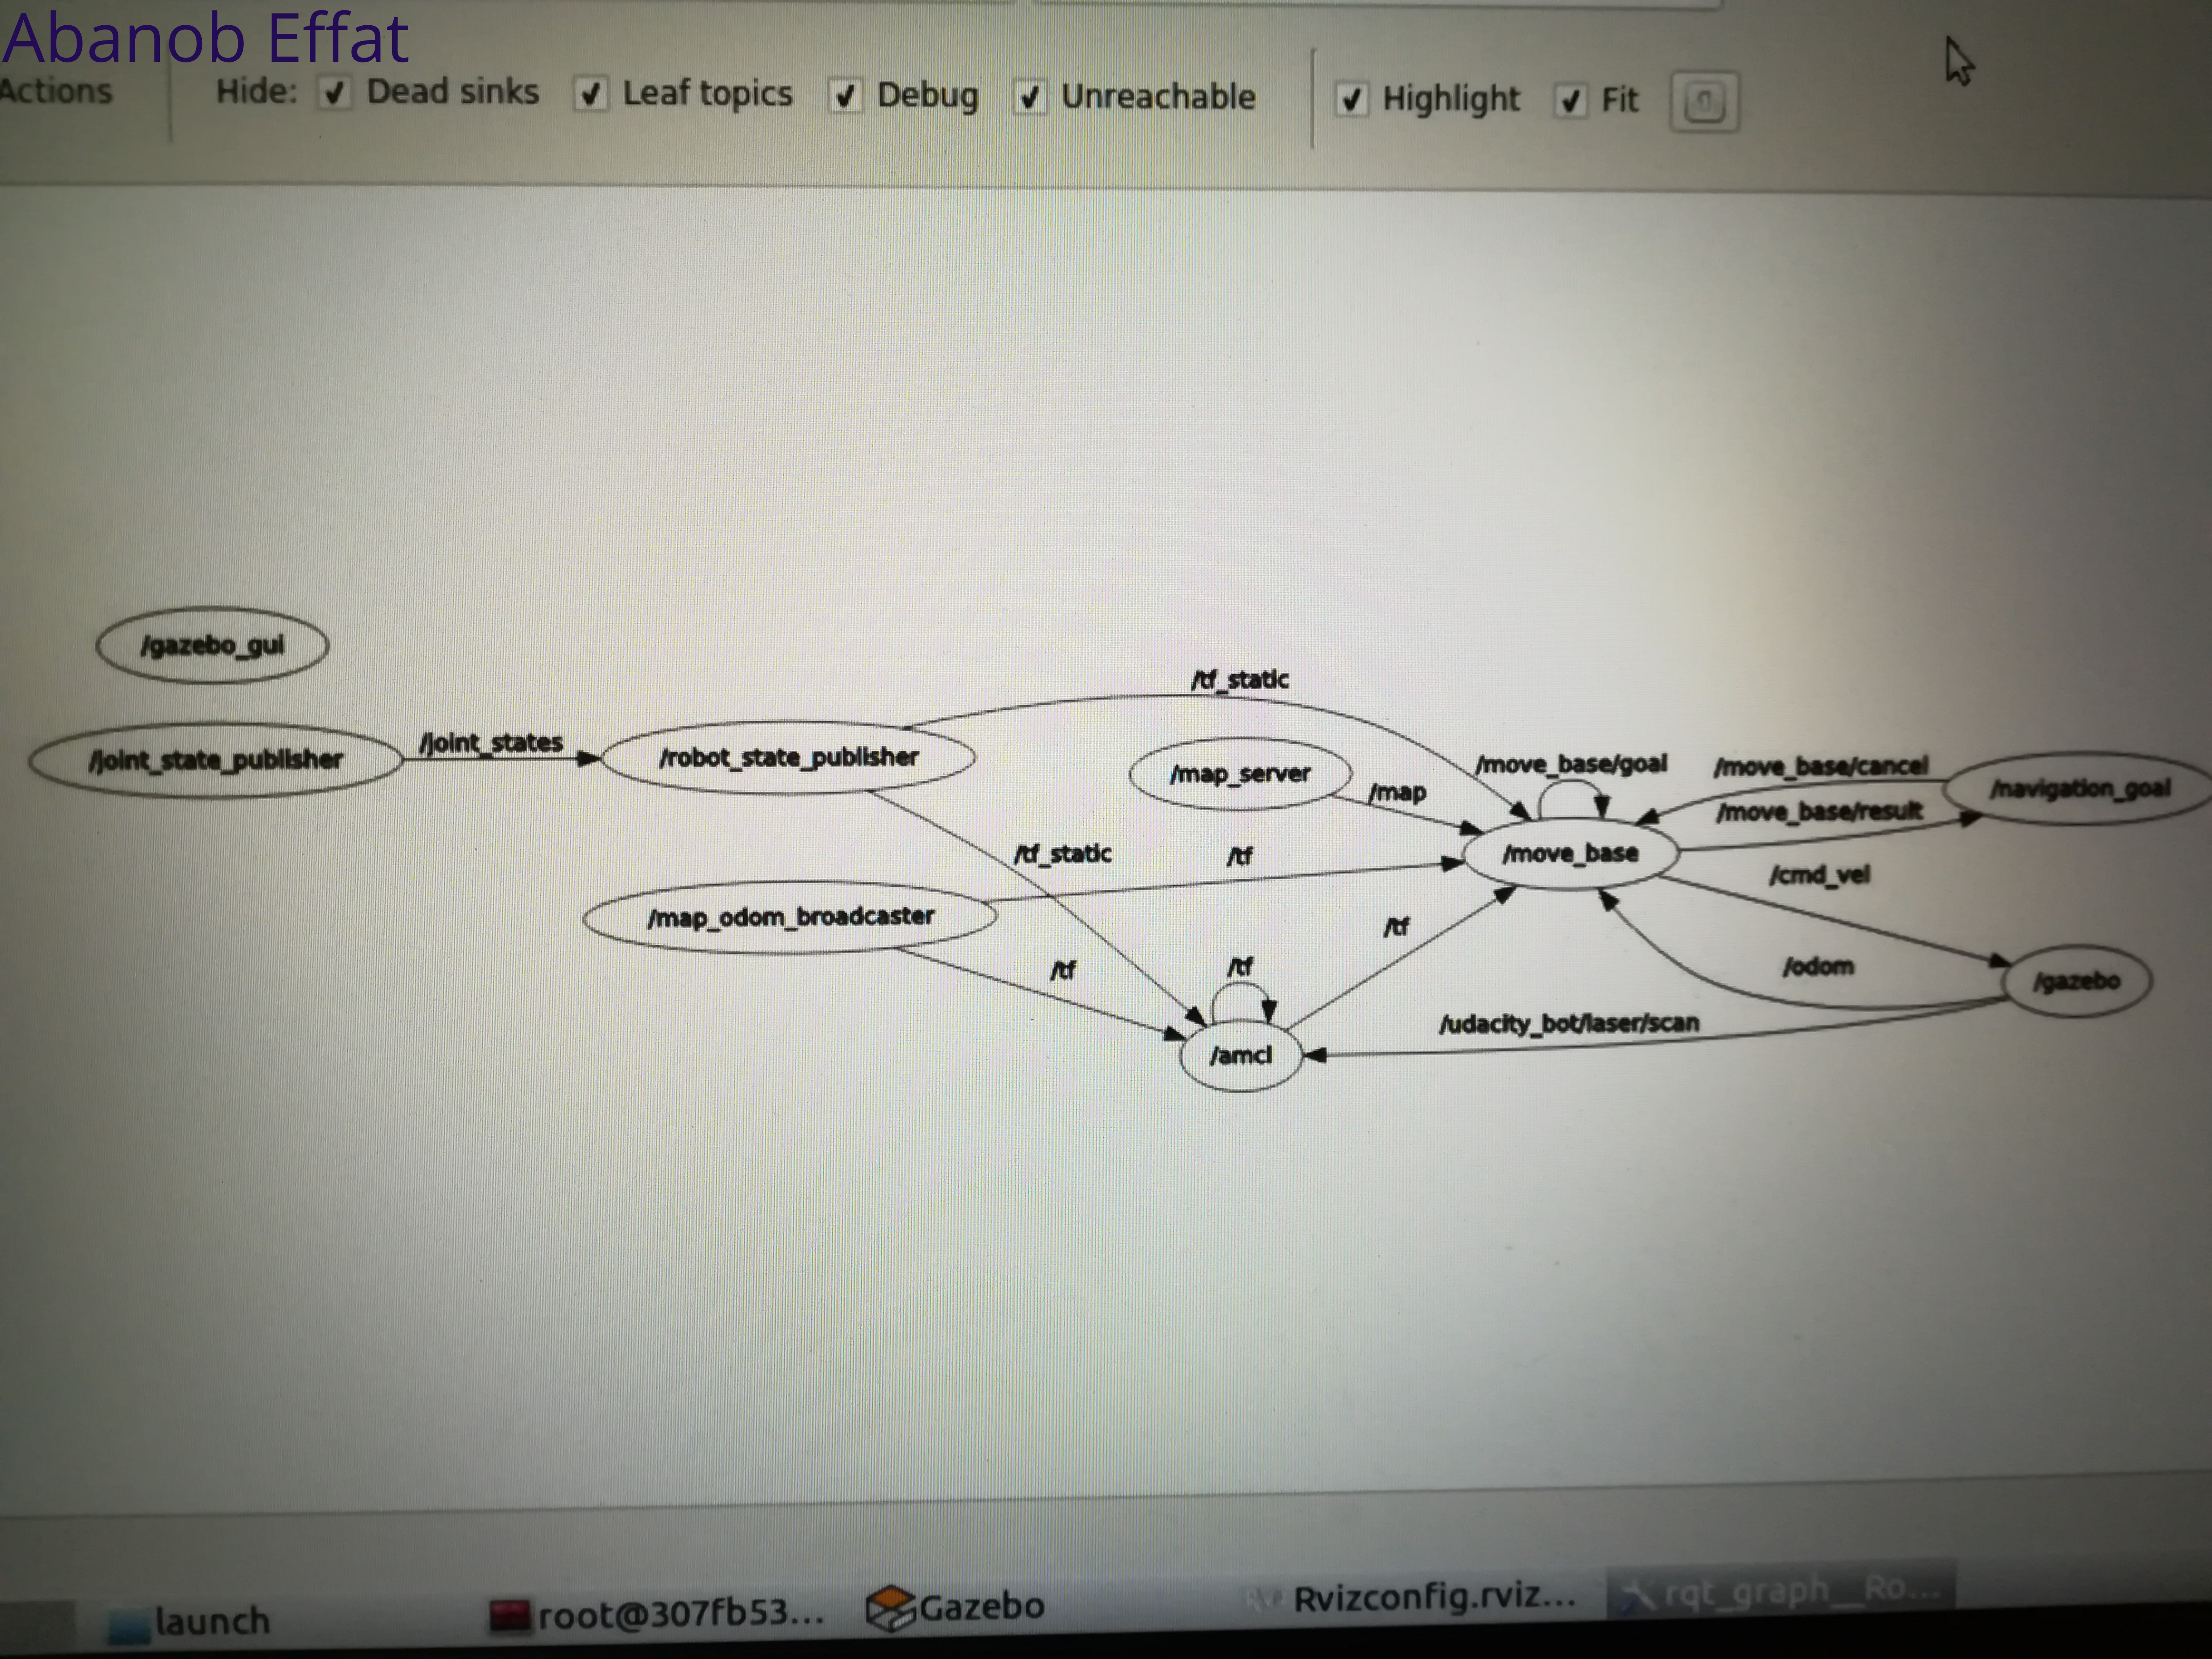
\includegraphics[width=\linewidth]{fig/node2.jpg}
      \caption{Udacity Graph}
\end{figure}

\section{Results}
\subsection{Localization Results}
At first i used 10 particles to 30 max and it made the robot go to the wrong path and wander a lot but after that i increased the particles to 100 as min and 1000 as max and that made the robot more efficient. 
\begin{figure}[thpb]
      \centering
      \includegraphics[width=\linewidth]{fig/fin_ubot.jpg}
      \caption{Udacity Goal}
\end{figure}
\begin{figure}[thpb]
      \centering
      \includegraphics[width=\linewidth]{fig/fin_u.jpg}
      \caption{Bot Goal}
\end{figure}

\subsection{Technical Comparison} % only facts
The main difference between the two robot models is the link, and the sensors position. There are differences in the selected parameters, which can be seen from the provided table. My bot  performed better because of the parameter tuning that was applied to it.

\section{Discussion}
The two robot models were able to reach the target. The Udacity Bot first went to opposite direction, while bot directly moved to the goal direction. The reason for this difference was the differently set parameters.

The convergence time for both of the robots were quite similar. Which shows that the AMCL package parameters were almost the same. Actually, only the number of particles parameter was different. As a result, these parameters do not have much effect on localization performance.

\subsection{Topics}
\begin{itemize}
\item bot performed better. It took less time to reach the goal position.
\item The different costmap parameters let bot to perform better. The bot directly started following the global path.
\item The 'Kidnapped Robot' problem is randomly moving the robot to another location. Both robots will fail to overcome this problem maybe if there is an algorithm that was applied to detect the kidnapping and decide a new plan this will solve this problem. 
\item Localization can be performed in scenarios in which the map is known, and the location of the robot does not randomly change.
\item MCL/AMCL algorithms were the best choice in small known environment as the particles are few but in large environment more particles are used and that could lead to a heavy computational crisis!
\end {itemize}

\section{Conclusion / Future work}
Both robots could reach their goal the bot robot could reach it faster, however for future work one can see that both robot lacks a commercial goal and it can be fixed if we applied some changes in the body design maybe to add a robot arm, or some sort of a flat box to act like a moving table which can be helpful in warehouses. Also modify the AMCL algorithm to solve the kidnapping problem.

\subsection{Modifications for Improvement}
Examples:
\begin{itemize}
\item Use three wheels instead of two
\item use two laser sensors
\end{itemize}





\bibliography{bib}
\bibliographystyle{ieeetr}

\end{document}